\documentclass{article}
\usepackage[affil-it]{authblk}
\usepackage{graphicx}
\usepackage[space]{grffile}
\usepackage{latexsym}
\usepackage{amsfonts,amsmath,amssymb}
\usepackage{url}
\usepackage[utf8]{inputenc}
\usepackage{hyperref}
\hypersetup{colorlinks=false,pdfborder={0 0 0}}
\usepackage{textcomp}
\usepackage{longtable}
\usepackage{multirow,booktabs}
\usepackage{todonotes}
\usepackage[xindy]{glossaries}
\usepackage{units}


\newcommand{\itemt}[1]{\item \textbf{#1}}
\newcommand{\um}{$\mu$m}

\makeglossaries

\newacronym{SMC}{SMC}{Sensor Mount Card}
\newacronym{BPB}{BPB}{Back-Plane Board}
\newacronym{APC}{APC128}{Analog Pipeline Chip 128}
\newacronym{SNR}{SNR}{Signal-to-Noise Ratio}
\newacronym{SEU}{SEU}{Single-Event Upset}
\newacronym{CMS}{CMS}{Compact Muon Solenoid}
\newacronym{VFPIX}{VFPIX}{Very Forward Pixel}
\newacronym{LHC}{LHC}{Large Hadron Collider}



\begin{document}

\title{VFPIX Silicon Telescope \\ Design Document}
\author{Caleb Fangmeier}
\author{Frank Meier}
\affil{Univ.\ of Nebraska-Lincoln}

\date{\today}


\maketitle

\begin{abstract}
  A silicon strip detector based telescope is being designed for the purpose of testing a under-development silicon pixel detector for the VFPIX upgrade of CMS.

  Here is documented the goals, constraints, and design decisions of the telescope.
\end{abstract}

\listoftodos

\newpage

\tableofcontents

\newpage

\section{Introduction}
The \gls{CMS} detector at CERN will undergo a second phase of upgrades during (year)\todo{Year of Phase II install}. A significant part of this upgrade will be the installation of the \gls{VFPIX} Detector. The \gls{VFPIX} Detector is being designed to cover the range of $\eta>2.5$\cite{Dominguez2013}. To give adequate resolution of relevant physics parameters a new pixel shape is being proposed. As part of the R\&D effort to design this new detector, a high resolution telescope is being built.

\section{Overview of Previous Work}
\label{sec:PreviousWork}
This project is an iteration and redesign of an existing telescope. Previous work\cite{Turner2012} has been done to design a versatile \gls{SMC}/\gls{BPB} with features including the ability to chain multiple \gls{BPB}s together to add aditional legs to the telescope. The \gls{SMC}, in particular, was well designed to allow the sensor strips to oriented $\pm45^o$ with respect to the plane of the \gls{BPB}. This allows different sensors strips to be oriented either parallel or perpendicular to each other. The same telescope hardware can then be configured to measure to various degrees either vertical or horizontal accuracy by flipping the \gls{SMC}s so the sensor strips align with either axis. This general design will be kept for the next iteration of the telescope, however the \gls{SMC}s themselves will be iterated upon as described in \ref{sec:HardProp:SMC}.

Work has also been done to improve the readout properties of the \gls{APC} chips.\cite{Ryser2013} The \gls{APC} has the unfortunate problem of a relatively weak output that has trouble driving a readout line at high frequencies. A proposed solution was to add a simple emitter-follower circuit on the BPB to reduce the load on the \gls{APC} output and drive the line going to the ADCs with the transistor. This resulted in an improved readout speed of 250ns per channel. It is hoped that by using a dedicated differential line-driver instead of the basic emitter-follower, an even better readout speed can be achieved(see sec. \ref{sec:PerformanceTargets}). 

It has also been discovered that there is significant variation between APCs where, all other things being equal, the output levels will vary from chip to chip by as much as 50mV.\cite{Ryser2013} However, this can be compensated for by adjusting the value of the Aref input per chip.

The precision of a strip telescope with charge sharing can be dramatically imporoved by improving its \gls{SNR}. It has been demonstrated that by using a somewhat more complex readout pattern, wherein some background noise is removed by subtracting adjacent values in the readout pipeline, the \gls{SNR} can be increased to approximately 25.An improvement from the 5-10 seen without this trick.\cite{Ryser2013}


\section{System Components}
The telescope consists of the following main components.
\begin{enumerate}
  \itemt{Silicon Strip Sensor}
    The sensitive device used in the telescope is a Silicon Strip Sensor with strip pitch of \unit{25}{\um} and overall dimensions of . 
    \todo{Find documentation for strip sensors.}
  \itemt{Analog Pipeline Chip x128 (\gls{APC})}
    The \gls{APC} (fig. \ref{fig:APC128_Schematic}) is a silicon chip designed for reading out charge from Silicon strip sensors. Each \gls{APC} contains 128 channels. The sensor being used each have 512 strips. Therefore, each sensor requires four \gls{APC} chips to read them out. The \gls{APC}'s normal operation is as follows:

    A bit is shifted into the pipeline shift register. This allows the preamp (leftmost in the diagram) to push charge onto the $C_p$ capacitors proportional to the current pulse-height. After the bit has shifted through the pipeline, another bit is shifted in. This pattern continues until a trigger is recieved, at which point a bit is placed into the pipeline to enable the proper $C_p$ capacitor based on the trigger delay. This capacitor is then read back through the preamp and the charge gets placed on the $C_L$ capacitor. Finally, when the charge is on each of the 128 $C_L$ capacitors a bit is pushed into the readout shift-regiter which enables one channel at a time to serialize the output.

    \begin{figure}[h]
      \centering
      \includegraphics{./figures/APC128_Schematic.png}
      \caption{A schematic diagram of the \gls{APC} chip.}
      \label{fig:APC128_Schematic}
    \end{figure}

  \itemt{Sensor Mount Card (SMC)}
    The SMC holds the Strip Sensor, 4 \gls{APC}, and some auxillary components to facilitate the operation of the \gls{APC}.
  \itemt{Back-Plane Board (BPB)}
    The BPB holds four SMCs. Its job is to physically hold the SMCs in place as well as route the signals between the SMC and the TRB.
  \itemt{Telescope Readout Board (TRB)}
    The TRB is responsible for controlling the operation of the telescope. This means it must generate the control signals for the \gls{APC} chips as well as the ADCs that will digitize and serialize the data being read from the \gls{APC}s. It will also contain an FPGA with supporting hardware to allow it to communicate with a connected PC via a USB connection. It must also
\end{enumerate}

\section{Performance Targets}

\begin{itemize}
  \itemt{\gls{SNR}:} 40
  \itemt{Readout Speed:} 100ns/channel $\rightarrow$ 8kHz readout of entire telescope
  \itemt{Pipeline Speed:} 40MHz, will vary with source
\end{itemize}


\subsection{Precision/Accuracy Targets}
\label{sec:PerformanceTargets}
\todo{check precision targets}
For charactering pixel sensors with pixel pitch as small as \unit[25]{\um}, a tracking precision of better than \unit[1]{\um} is desired. To achieve this, we require a \gls{SNR} of better than 40.
\subsection{Speed Targets}

\section{Hardware Proposal}

\subsection{Silicon Strip Sensor}
The silicon micro-strip sensors that will be used to measure particle tracks in the telescope have 512 strips each. Fig. \ref{fig:Microstrip_Sensor} shows the layout of a sensor.

\begin{figure}[h]
  \centering
  \includegraphics{./figures/Microstrip_Sensor.png}
  \caption{Layout of a silicon micro-strip sensor. As shown, there are 25$\mu$m between strips. The strips are divided between 2 layers so the separation between strips on the same layer is 50$\mu$m}
  \label{fig:Microstrip_Sensor}
\end{figure}

\subsection{Analog Pipeline Chip}
The \gls{APC} will be used to read charge from the silicon strip sensor.

\subsection{Sensor Mount Card}
\label{sec:HardProp:SMC}

The design choices of the \gls{SMC} are especially critical becuase it is responsible for ensuring optimal operation of the \gls{APC} chips during both control and readout.

The readout of the \gls{APC} is analog so it is more susceptable to noise and interference than a digital signal would be.

The SMC will be subject to the highest radiation fluence of the entire system which limits the choices of hardware that can be placed on the it. Any FLASH memory dependent hardware will be subject to \gls{SEU}s.

Because of these restrictions, only the minimum hardware necessary to ensure high quality \gls{APC} operation and output will be placed on the SMC. This hardware consists of a 2-channel differential-line driver amp. The chosen amp is the ADA4950-2\cite{ADA4950}. Two of these will be placed on each SMC, as close as possible to the \gls{APC}s to minimize the capacitave load on the outputs.


It has been determined (see sec. \ref{sec:PreviousWork}) that to achieve optimal operation of each \gls{APC} in the telescope, it is important to be able to set each \gls{APC}s Aref voltage individually. To do this, four potentiometers will be placed on each SMC to allow for idividual calibration of each \gls{APC}s Aref value. Potentiometers were chosen for this task over DACs becuase of the risk of \gls{SEU}s in the DACs are placed near the beam, and the addition of many new signal lines if they are placed far from the beam.


\begin{figure}[h!]
  \centering
  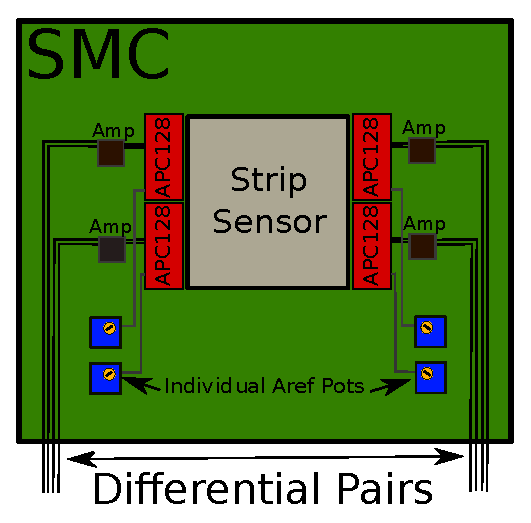
\includegraphics{./figures/SMC.eps}
  \caption{An illustration of the \gls{SMC}. Not shown: \gls{APC} control signals}
  \label{fig:SMC}
\end{figure}


\subsection{Back-Plane Board}

The primary jobs of the \gls{BPB} are to route signals between the \gls{TRB} and the \gls{SMC}s and hold the \gls{SMC}s in place. It has been considered to digitize the signals on the \gls{BPB} by placing the ADCs on it. However, this has two major drawbacks. First, since ADCs are stateful devices, they are susceptable to \gls{SEU}s
\todo{decide placement of ADCs, either on TRB or BPB}

\begin{figure}[h!]
  \centering
  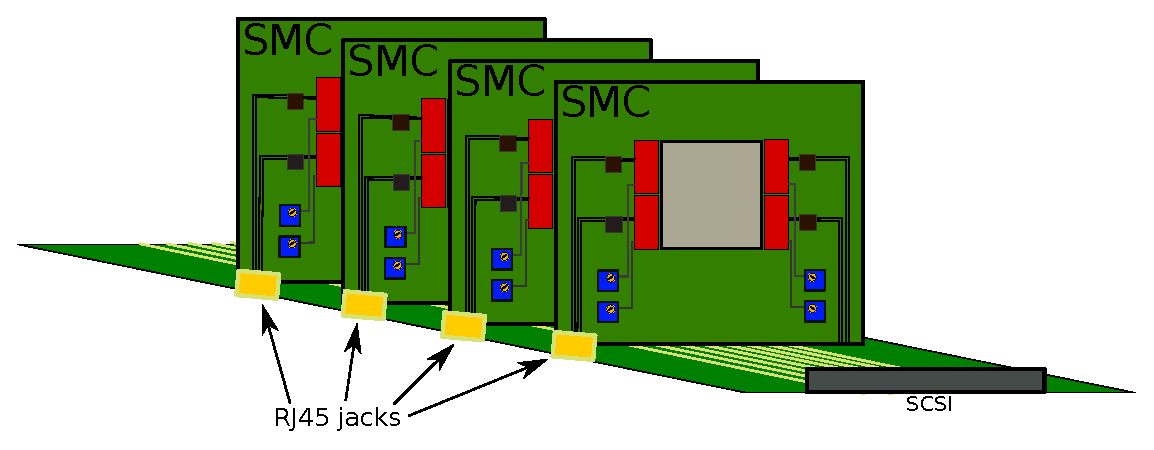
\includegraphics{./figures/BPB.eps}
  \caption{An illustration of the BPB}
  \label{fig:PBP}
\end{figure}

\subsection{Telescope Readout Board}
\missingfigure{\gls{TRB} Block diagram \& illustration}

\section{Timeline}
\todo{Fill in timeline}

\newpage
\bibliographystyle{plain}
\bibliography{references}

\glsaddall
\printglossaries

\end{document}
